

\question[3] Compute the area of the figure contained between the curves
\[ y = \dfrac{1}{1+x^2}\text{ and } y=\dfrac{x^2}{2} \]

\ifprintanswers
  \vspace{0.3cm}
  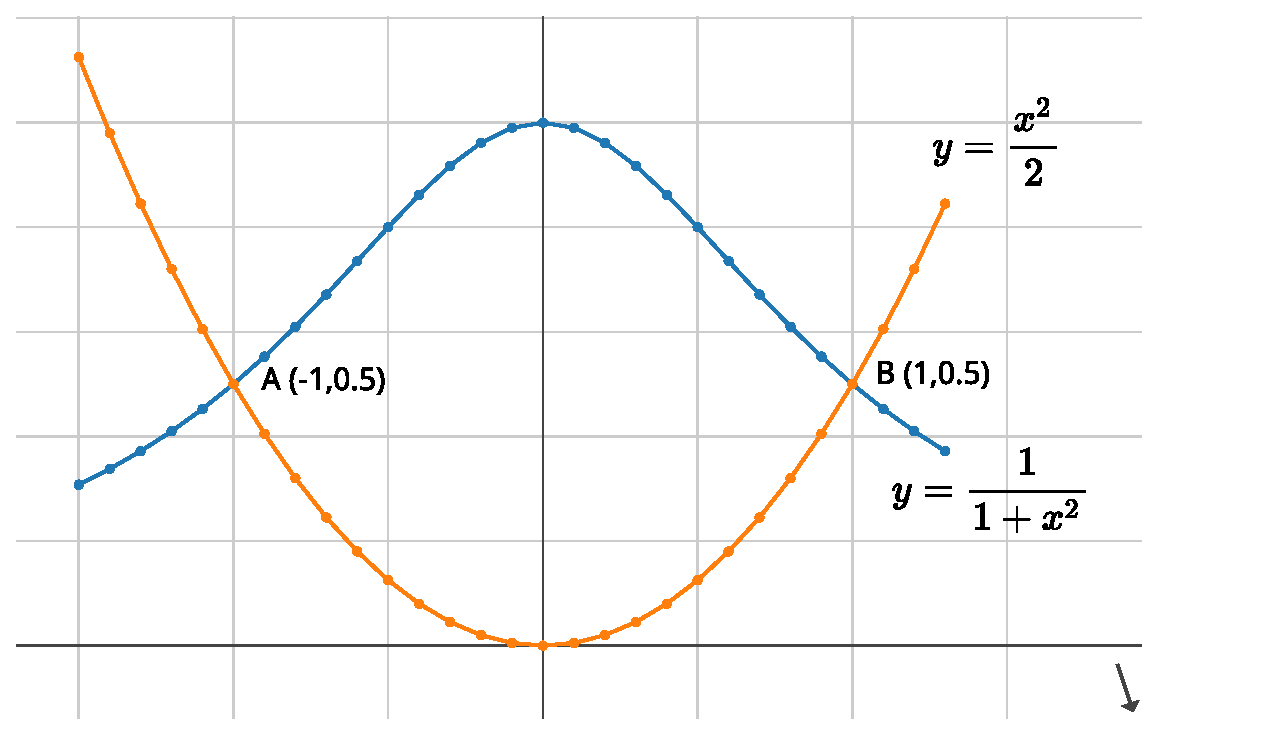
\includegraphics[width=300pt]{plotly.eps}
\fi

\begin{solution}[\fullpage]
	The two curves are as shown in the figure above. And they intersect when
  \begin{align}
     \dfrac{1}{1+x^2} &= \dfrac{x^2}{2} \\
     \implies x^4+x^2-2 &= 0 \\
     \text{Setting } z = x^2, \text{ we get }
     z^2+z-2 &= 0 \\
     \implies z = 1, -2
  \end{align}
  As $z = x^2$, it has to be > 0. And therefore, 
	\[ z = 1 \implies x = \pm 1 \]
	The required area $=R$ therefore is 
  \begin{align}
     R &= 2\cdot\left[ \int_{-1}^1 \dfrac{1}{1+x^2}\ud x - \int_{-1}^1\dfrac{x^2}{2}\ud x\right] \\
       &= \underbrace{2\cdot\left[ \int_0^1 \dfrac{1}{1+x^2}\ud x - \int_0^1\dfrac{x^2}{2}\ud x\right]}_{\text{due to symmetry}} \\
     &= 2\cdot\left[ \left( \tan^{-1} x\right)_0^1 - \left( \dfrac{x^3}{6}\right)_0^1\right] \\
     &= \dfrac{\pi}{2} - \dfrac{1}{3} 
  \end{align}
\end{solution}
\ifprintanswers\begin{codex}$\dfrac\pi{2}-\dfrac{1}{3}$\end{codex}\fi
